\begin{flushright} {\tiny {\color{gray} (tikz\_3x2\_Q2.tex)}} \end{flushright}
%~~~~~~~~~~~~~~~~~~~~~~~~~~~~~~~~~~~~~~~~~~~~~~~~~~~~~~~~~~~~~~~~~~~~~~~~~~~~~~~~~~~~~~~~~~~~~~~~~~

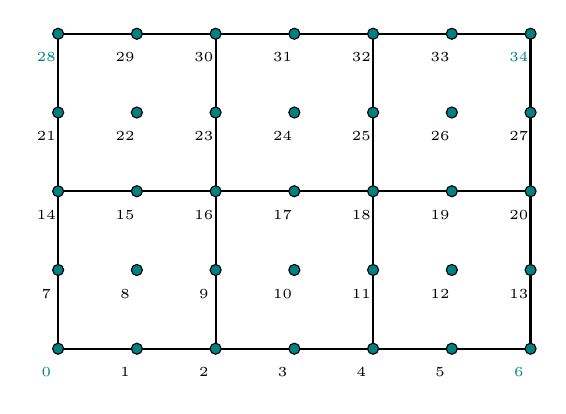
\begin{tikzpicture}
%\draw[step=0.5cm,gray,very thin] (0,0) grid (8,6); %background grid

\draw[thick] (1,1) -- (7,1) -- (7,5) -- (1,5) -- cycle;  
\draw[thick] (1,3) -- (7,3) ;
\draw[thick] (3,1) -- (3,5) ;
\draw[thick] (5,1) -- (5,5) ;

\draw[black,fill=teal] (1,1)     circle (2pt); 
\draw[black,fill=teal] (2,1)     circle (2pt); 
\draw[black,fill=teal] (3,1)     circle (2pt); 
\draw[black,fill=teal] (4,1)     circle (2pt); 
\draw[black,fill=teal] (5,1)     circle (2pt); 
\draw[black,fill=teal] (6,1)     circle (2pt); 
\draw[black,fill=teal] (7,1)     circle (2pt); 

\draw[black,fill=teal] (1,2)     circle (2pt); 
\draw[black,fill=teal] (2,2)     circle (2pt); 
\draw[black,fill=teal] (3,2)     circle (2pt); 
\draw[black,fill=teal] (4,2)     circle (2pt); 
\draw[black,fill=teal] (5,2)     circle (2pt); 
\draw[black,fill=teal] (6,2)     circle (2pt); 
\draw[black,fill=teal] (7,2)     circle (2pt); 

\draw[black,fill=teal] (1,3)     circle (2pt); 
\draw[black,fill=teal] (2,3)     circle (2pt); 
\draw[black,fill=teal] (3,3)     circle (2pt); 
\draw[black,fill=teal] (4,3)     circle (2pt); 
\draw[black,fill=teal] (5,3)     circle (2pt); 
\draw[black,fill=teal] (6,3)     circle (2pt); 
\draw[black,fill=teal] (7,3)     circle (2pt); 

\draw[black,fill=teal] (1,4)     circle (2pt); 
\draw[black,fill=teal] (2,4)     circle (2pt); 
\draw[black,fill=teal] (3,4)     circle (2pt); 
\draw[black,fill=teal] (4,4)     circle (2pt); 
\draw[black,fill=teal] (5,4)     circle (2pt); 
\draw[black,fill=teal] (6,4)     circle (2pt); 
\draw[black,fill=teal] (7,4)     circle (2pt); 

\draw[black,fill=teal] (1,5)     circle (2pt); 
\draw[black,fill=teal] (2,5)     circle (2pt); 
\draw[black,fill=teal] (3,5)     circle (2pt); 
\draw[black,fill=teal] (4,5)     circle (2pt); 
\draw[black,fill=teal] (5,5)     circle (2pt); 
\draw[black,fill=teal] (6,5)     circle (2pt); 
\draw[black,fill=teal] (7,5)     circle (2pt); 

\node[] at (0.85,0.7) {\tiny \color{teal} 0};
\node[] at (1.85,0.7) {\tiny 1};
\node[] at (2.85,0.7) {\tiny 2};
\node[] at (3.85,0.7) {\tiny 3};
\node[] at (4.85,0.7) {\tiny 4};
\node[] at (5.85,0.7) {\tiny 5};
\node[] at (6.85,0.7) {\tiny \color{teal} 6};

\node[] at (0.85,1.7) {\tiny 7};
\node[] at (1.85,1.7) {\tiny 8};
\node[] at (2.85,1.7) {\tiny 9};
\node[] at (3.85,1.7) {\tiny 10};
\node[] at (4.85,1.7) {\tiny 11};
\node[] at (5.85,1.7) {\tiny 12};
\node[] at (6.85,1.7) {\tiny 13};

\node[] at (0.85,2.7) {\tiny 14}; 
\node[] at (1.85,2.7) {\tiny 15}; 
\node[] at (2.85,2.7) {\tiny 16}; 
\node[] at (3.85,2.7) {\tiny 17}; 
\node[] at (4.85,2.7) {\tiny 18}; 
\node[] at (5.85,2.7) {\tiny 19}; 
\node[] at (6.85,2.7) {\tiny 20}; 

\node[] at (0.85,3.7) {\tiny 21}; 
\node[] at (1.85,3.7) {\tiny 22}; 
\node[] at (2.85,3.7) {\tiny 23}; 
\node[] at (3.85,3.7) {\tiny 24}; 
\node[] at (4.85,3.7) {\tiny 25}; 
\node[] at (5.85,3.7) {\tiny 26}; 
\node[] at (6.85,3.7) {\tiny 27}; 

\node[] at (0.85,4.7) {\tiny \color{teal} 28}; 
\node[] at (1.85,4.7) {\tiny 29}; 
\node[] at (2.85,4.7) {\tiny 30}; 
\node[] at (3.85,4.7) {\tiny 31}; 
\node[] at (4.85,4.7) {\tiny 32}; 
\node[] at (5.85,4.7) {\tiny 33}; 
\node[] at (6.85,4.7) {\tiny \color{teal} 34}; 

\end{tikzpicture}

